% !Mode:: "TeX:UTF-8"

\chapter[并行计算简介]{并行计算简介}
\section{并行计算产生的背景}

在社会需求和技术更新迭代的推动和促进下,高性能计算成为许许多多应用应用领域的必须。
许多应用领域,如生物计算,卫星云图计算,基因对比,经济金融计算,股票交易等等领域对计算能力需求已越来越高,这
大规模的大数据量计算需要刺激和激发了大规模并行计算的流行和兴起,对并行计算提出了更多的要求
,但是曾经还缺乏标准的支持,出现并行计算标准混乱的情况。其实,并行是终必将在所有计算机中展现出来—
—包括个人数字助理、PC计算机、工作站,计算集群及超级计算机等。

计算机的出现深刻了影响了现代科技,世界经济发展,文化生活,加快在人类生活学习工作的各个脚步,
计算机的迅猛发展也带动了其他学科的快速发展。随着网络技术、计算机科学,计算机理论的快速发展
计算机对经济与科技生活的影响日益深入,刺激和引发了更多的计算需求,反过来促进和推动了高性能计
算技术。现代自然科学甚至社会科学参与的各领域,如:计算流体力学、 计算结构力学、生物医学、人工智能及模式识别、
量子化学、核磁共振、密码破译等,对高性能计算的需求开始逐渐显现。

1992年初,美国高性能计算与通信计划(HPCC)提出了在科学与工程计算领域中对国民经济与国
家安全都具有深远影响的一些重大挑战性课题,其中包括全球气候变化、长期天气预报、海洋环流建模、
湍流分析、空气动力学、三维生物结构、三维等离子体研究、四维时空结构、催化剂设计、药物分子结构设计、结
构生物学、人体基因与遗传工程、数字剖析、图像理解等方面 \cite{Daibo} 。每一个课题都适合使用并行计算处理,同时
每一个重大课题无不涉及到了极大的计算量,无一不对计算机性能提出了高要求。

举例来说,全球气象中期天气预报要求在24小时内完成48小时天气预测数值模拟,至少需要635万个网格点,内存需求大于1T,计算性能
要求高达25万亿/次,而传统的单机技术能力较弱,与大量的计算数据需求执行形成了极大的矛盾,形成新的并行计算标准势在必行
计算机必将走向并行发展的道路,海量数据的计算需求必将成为推动并行机体系结构不断向前发展和演进的原超级力。

并行计算与并行算法是计算数学和新一代的计算机结合的产物,为了能够在尽量短的时间实现大量
大型数值计算问题的,不仅仅需要功能完善的并行,还需要合理的,能够在并行机上应用的合理的并行算法。 
并行计算给了解决打计算量问题的新的思路,并行计算功能强大,性能强大,规模强大,具有巨大的
数值计算和数据处理能力,能够对社会带来巨大的经济效益。总结而言,并行计算机是由多个处理器组成,相对于串行计算机只有单个处理器的情况
而言,能够高效,高效率地进行复杂问题计算的计算机系统,并行计算机能够在同一时间内执行多条指令,或处理多个数据的计算。  

并行计算的研究目的主要是将复杂问题并行分解为可被多个小部分解决的子问题,后将这些小问题分配
由多个计算机结点以进行并行处理,最后汇集各个计算结点的计算结果最后综合起来以得到最终结果。
总而言之,并行计算是为了加快运算速度和解决大主存容量的求解问题,而发展起来的多计算机/多处理机的并行编程技术。并行计算
解决问题的算法如图~\ref{fig:parallel}
    \begin{figure}[htbp]
    \centering
    \includegraphics[width=0.8\textwidth]{parallel}
    \caption{并行计算算法示意图}\label{fig:parallel}
    \vspace{\baselineskip}
    \end{figure}



并行处理技术的诞生和进一步的发展,正是相应了时代的召唤,适应了大数据量的计算需求,尤其是在当今
云计算的背景下。

\section{并行计算发展}
    
\subsection{并行计算发展历程}
并行计算技术的发展先后经历了以下几个阶段:

60年代中期,先后诞生了以鲍勒斯公司的ILLAC-IV为代表的单指令流多数据流的阵列处理机和以
CDC公司的STAR-100、CRAY公司的CRAY-1为代表的单处理机多流水线向量机。同时,我国也诞生了YH-1巨型机。
微程序控制的计算机开始普及。为了减小CPU和主存储器之间的速度差距,计算机采用了流水线和高速缓存;
同时为了使CPU和I/O操作在支持多用户程序和多任务管理,开始提供多道程序的支持。

70年代开始,在计算机硬件层面,出现分布存储器、共享存储器和向量硬件选件的不同结构的并行计算机,同时在软件层面,
为了满足并行计算处理需求的多处理操作系统开始发展,操作系统平台上对应的多处理器编程语言和编译器应运而生,
用于并行处理的软件工具和环境日益完善。SMP方式的总线协议,出现了共享主存的并行多处理系统(SPP机)。这
段时期的代表系统:CrayX-MP,IBM/3090VF,VAX9000,BBNTC-2000等。SPP类型的YH-2和曙光-I机型也开始
出现。并行处理技术在70年代开始逐渐成熟发展。

1972,超级计算机ILLIAC-IV的诞生,标志这大规模并行处理机(MPP)的兴起,其本身更成为并行处理的模范样本。
二以CRAY为代表的向量机由于天然良好的可编程性,仍然占据主流市场。 

 80年代中期,产生了共享存储多处理机Shared-Memory MultiProcessor,在一个计算机上汇集一组处理器,处理器之间通过共享内存来进行通信,
由单一的操作系统进行作业管理,极大了提高了整个系统的计算能力和吞吐量。80年代后期,向量机的造价成本上升,然而性能的提高却无法随着
造价的提高而直线提高,导致MPP替代向量机称为主流的并行计算技术,MPP体系结构示意图如图~\ref{fig:mpp}。MPP系统具有可伸缩性和可容时延性,性价比高的特点,采用了砷
化嫁技术、VLSI硅片、高密度组装,光技术等先进技术。Thinking Machines公司的CM-5和Paragon是当时MPP系统的代表,我国当时的代表性
产品为神舟-II巨型机。

    \begin{figure}[htbp]
    \centering
    \includegraphics[width=0.9\textwidth]{mpp}
    \caption{mpp体系结构示意图}\label{fig:mpp}
    \vspace{\baselineskip}
    \end{figure}
    
90年代,整个并行计算机的体系结构框架趋于统一,DSM(Distributed Shared Memory)分布式共享存储,MPP(Massively Parallel Processing)
大规模并行处理结构,NOW(Network of Workstations)工作站集群各种体系架构趋向一致。期间也出现了三种架构的组合架构,三者之间的界限
也越来越模糊。

    进入二十一世纪,并行计算系统在进一步发展和壮大,硬件方面,单个节点的处理性能更高,并行计算节点之间互连方式和结构也在优化
和改进。基于NUMA方式构成的分布共享存储器组成的并行机系统,具有良好的可伸缩性和可编程性,称为未来一个重要发展方向。同时,
随着快速以太网等局域网络技术的不断进步,由高性能微机和工作站组成的计算机机群(Cluster)进行并行计算的也成为现阶段并行计算
研究的重要一部分。

\subsection{并行计算发展现状}
    并行计算的研究目前主要集中在并行计算的硬件平台(并行计算机),理论研究(并行算法),软件支撑(并行程序设计)应用研究和几个方面。在
理论研究方面,主要是研究并行程序的描述,体系结构,设
计与实现并行算法,负载均衡等方面。在并行计算的应用研究方面,正在努力让并行算法实现良好的可移植性,形成一次编译,到处运行
的优势,设计出稳定高效的硬件设备,通信设备;解决和降低执行并行程序时处理器之间的相互通讯问题,减小和优化通信开销。在并行程
序设计方面,主要研究如何运用现有的编程语言和软件环境,分解原串行程序的问题,分治到多个计算结点上,以满足大规模并行应用的需
要\cite{Chenguoliang}。

    并行计算研究目前存在的几个问题
    \begin{itemize}   
    \item 并行算法研究热度不够
    \item 大部分并行计算应用的效率依然不够高,无法充分利用并行计算机的资源
    \item 并行编程语言对计算机编程人员不够透明,难度依然较高,同时缺乏高效的并行编程环境
    \item 并行计算机本身存在耗能高,管理困分,可扩展性差等方面的问题
    \end{itemize}

总体来说,并行软件和并行算法的发展远远落后于并行计算机系统的发展。综上所述,并行计算机的发展趋势是:

\begin{enumerate}
\item 并行计算技术的潮流是软件硬件一体化。
\item 并行计算技术中的并行软件支撑和理论研究成为限制并行计算进一步发展的主要瓶颈。
\item SMP由于共享内存结构的限制,只能局限于特定的应用场景。
\item 由于向量机和MPP的研制费用高,性价比低等诸多因素影响,市场缩小。
\item 由高性能微机或者工作站,PC通过高速网络互联而成的机群,将因为具有超高性价比,投资风险小,可扩展性好,和优良的计算性能,
可集成现有软硬件资源,开发周期段,可编程性强等诸多优点,配合日渐成熟可移植异构编程环境PVM和标准的消息传送平台MPI,
成为并行计算技术中举足轻重的一环。
\end{enumerate}

\subsection{国内外并行计算发展现状}
    并行计算机由于具有计算性能强大,可用性强等特点,具有超级的数值计算和数据处理能力,被广泛应用于经济建设,科技建设,
科学研究,天气预报,武器制造,虚拟现实等领域中。并行计算技术的发展水平也已经称为一个国家综合实力的标志,对保卫国家安全,
全面促进科研水平的进步,推动经济的发展有着举足轻重的作用。
    
    美国在并行计算研究领域,一直处于领先的地方,从之前的MPP系统架构已经转向了具有可伸缩性的并行机和各种类型的计算机集群。
计算机集群可以利用部门和单位已经具备的局域网环境,PC机,工作站,服务器等在并行系统软件的组建下,构成计算机集群,成本非常低。
美国计算机厂商对由NUMA,尤其是CC-NUMA方式构成的可伸缩并行机系统特别看好。SGI公司推出了可伸缩共享内存多处理器结构,采用MIPS
R10000 4路超标量处理器。每个结点由多个CPU,一定容量的存储器,I/O和相应的硬件组成。Sequent公司则用传统SMP多机系统作为结点机,
最小的机器内部有4个Pentium Pro超标量机以及相应的存储槽和PCI槽,每个结点称为Quad,更大多的Quad使用高速IQ Link连接器连接起来,
形成规模可伸缩的CC-NUMA并行及系统。在计算机集群方面的研究工作,美国研究有2个侧重点:一个侧重点时如何减少结点机间的通信开销
第二个侧重点是有关于计算机集群的环境,前者主要使用新的高速网络如ATM,快速Ethernet,FDDI等,后者对应的重点时设计新的精简通信
协议,减少传统通信协议的层次,其他涉及的有编程环境,任务调度,负载均衡等等程序设计方面的工作。

    德国的科学研究机构意识到推广并行应用的意义,研究重点为并行应用,并行编程环境,优化技术和开发工具等等方面。过去德国曾
着重研究MPP系统,采用了微内核架构,微内核的功能和大小可相应伸缩,因此,能大大减小操作系统介入通信时所需的开销。柏林计算机研究所
曾成功研制出MANNA并行机,采用了快速,多层次架构的纵横较差开关互联网络。

    日本在90年代推出了现实世界计算计划以来,没有产生太多的成果,其在光计算机和大规模神经网络计算机系统方面的工作遇到了很大的瓶颈。


    我国计算机技术起点低,起步晚,而且西方发到国家奉行高性能技术不出口政策,在高性能计算机方面对我国实行严格禁运
措施,加上计算机教育起步的落后,总体导致了我国现在的并行计算机技术相对落后。而且,作为高性能计算机核心部件的CPU,
我国最初没有自主创造的能力,国产CPU龙芯的出现打破了这一局面,即使性能还不够出众,但标志着我国已经在研制具有完全自主知识产
权的高性能计算机CPU上迈出了重要的一步。进来,我国中国科学院自主开发和研制了一系列的曙光高性能计算机,拥有了世界前五计
算能力的银河计算机,这些历史性的跨越使我国成为少数具有自主开发和生产高性能计算机能力的国家之一。

    即使我国已经作出了很多的研究和努力,但我国的并行计算机技术的研究和应用的成效相对于计算机发达国家相比,还存在着较大的
差距,有待进一步提高和发展。美日欧等发达国家的科技企业、国防部门和科学研究部门,如MIT,哈佛医学院,NASA,天气预报中心等等都在
使用高性能并行计算,已经有多年的使用经验。而我国高性能计算的应用才刚刚迈进应用部门和科研部门的门槛,还缺乏足够有效的使用经验,
但相信随着政府对超级计算机研制的支持力度加强,科研院所对并行计算的重视,一定会有不错的发展前景\cite{Zhangzhihong}。

\section{并行计算平台}
    并行计算需要系统软件方面的支撑,常见的并行计算平台使用的大部分操作系统都采用了开源免费的Linux操作系统,在硬件支撑方面则
属于百花齐放的状态,在并行计算算法理论设计方面也有各种编程模式可供使用。

\subsection{并行计算软件-Linux操作系统}
    Linux操作系统是一种自由和开放的操作系统,其目标是类Unix。Linux操作系统原为Linux内核,由Linus Torvalds在1991年10月5号发布.
本身linux仅仅代表Linux内核,在包含进更多的GUI组件和其他许多使用工具后,成为完整的Linux操作系统。

    Linux被移植到了很多计算机硬件平台,具有优秀的可移植性.Linux同时作为一个领先的操作系统,
可以运行在服务器或者其他大型平台上,如大型主机和超级计算机.世界上的TOP500超级计算机采用
的都是Linux发行版.同时Linux系统也被移植到广大的嵌入式系统上,很多电视机盒,手机操作系统等等
都采用的是Linux操作系统。

    Linux操作系统采用的GNU通用公共许可证,任何人和机构都可以自由地使用Linux的所有底层源代码
,也可以自由地修改和再发布.1993年Richard Stallman发起GNU计划,制造出了c编译器,GNU C库和基本的命令行使用程序
。Linus Torvalds 和Richard Stallman合作推出了Linux,形成了一套完整的操作系统,自由软件基金会提议
将组合系统命名为GNU/Linux,包含了大量的GNU软件,包括一个Shell程序,必要的libc函数库,c/c++
编译器和工具等等。现在,在Linus Torvalds的领导下,全世界众多的开发者都在共同参与开发Linux内核,而richard 
Stallman领导的自由软件基金会则继续提供大量的可以在Linux内核上使用的。

    Linux具有设备独立性,内核具有强大的适应力,能够给系统提供更高的可靠性.Linux发行版一直在被用来做
服务器的操作系统,并且独占奥头,许多云服务器公司都在使用Linux操作系统作为其基础软件部分的
一部分,其也经常做为超级计算机和并行计算机群的操作系统。
    
    Linux系统的特点:
    \begin{itemize}
    \item 开放性:Linux系统遵循国际POSIX标准,可以在遵循此标准的软件和硬件上使用,实现兼容,
方便的互连,同时Linux操作系统是开放内核源代码的,方便各种用户和商业用户进行改革。
    \item 多用户:系统资源可以被不同的用户各自使用,每个用户对自己的资源,如文件,设备等等
进行控制,拥有自己的用户空间。    
    \item 多任务:计算机可以同时执行多个程序,程序之间不会相互影响.Linux采用抢占调度的多任务方式
,用户可以充分利用计算机软硬件资源。
    \item 先进的网络功能,Linux是较早支持TCP/IP协议的操作系统之一,在网络通信方面优于其他
操作系统,内涵文件传输协议和远程访问。
    \item 可靠的安全性:Linux内涵了多种安全技术措施,包括对用户的读,写权限控制,内核空间和
用户空间的分离,各用户之间的隔离,提供了许多必要的安全保障。
    \item 良好的移植性: 能够从微机,嵌入式版本到大型计算机的任何环境和平台上运行,为不同的计算机平台
与其他机器进行准确,有效的通信提供了手段。
    \end{itemize}

    Linux众多的优点让其称为并行计算技术中不可获取的一部分,下图~\ref{fig:linux}为世界前500强超级计算机采用操作系统的统计情况,截至时间06/2009
    \begin{figure}[htbp]
    \centering
    \includegraphics[width=0.9\textwidth]{linux}
    \caption{超级计算机使用操作系统统计}\label{fig:linux}
    \vspace{\baselineskip}
    \end{figure}

\subsection{并行计算-程序设计}
    目前,并行程序设计常用3种环境,可以分为三类:消息传递,共享存储,数据并行,
下表为各个并行编程环境的简单介绍:

    \begin{table}[htbp]
    \centering  % 表居中
    \begin{tabular}{lccc}  % {lccc} 表示各列元素对齐方式,left-l,right-r,center-c
    \hline
    特征&消息传递&共享存储&数据并行\\ \hline 
    典型特征&MPI,PVM&OpenMP&HPF\\        
    可移植性&所有流行并行机&SMP,DSM&SMP,DSM,MPP\\      
    并行粒度&进程级大粒度&线程级大粒度&进程级细粒度\\     
    并行操作方式&异步&异步&松散同步\\   
    数据存储模式&分布式存储&共享存储&共享存储\\
    数据分配方式&显示&隐式&半隐式\\
    入门难度&较难&容易&简单 \\
    扩展性&好&较差&一般\\ \hline
    \end{tabular}
    \caption{三种并行编程环境的主要特征}
    \end{table}

    MPI(Message Passing Interface)是基于消息传递的并行编程模型。并行执行的各个进程具有独立的堆栈和代码栈,作为互补相关的
多个程序独立执行,进程间的通信通过显示地调用通信函数完成。其时间消耗主要时通信自身的时间,还有消息传递本身消耗的时间\cite{Zhangwusheng}。

    PVM时运行于网络情况下的虚拟并行机系统的软件包,将网络环境下Unix和Linux操作系统的计算机虚拟成为一个单一的并行虚拟机。PVN
支持用户采集消息传递方式编写程序,以任务为单位,即Unix进程。PVM支持在虚拟机自动加载任务运行,各个任务之间可以传递消息和进行
同步\cite{Wanglei}。

    OpenMP是一种面向共享内存及分布式共享内存的多处理器多线程并行编程语言,能够显示指导多线程和共享内存并行的应用程序.OpenMP
底层采用线程,需要在程序中显示地通过编译语言控制程序的并行化。程序流程采用Fork-Join模式,起初程序只有一个主进程存在,当有计算
任务到达时,Fork出一个子线程来执行计算任务。此时,主进程和子线程同时工作,在子线程推出后,主进程继续其工作。下
图~\ref{fig:openmp},为OpenMP的Fork-join模型。主进程产生4个工作子线程,等待4个子线程完成任务后汇合到主进程,主进程之后推出。

    \begin{figure}[htbp]
    \centering
    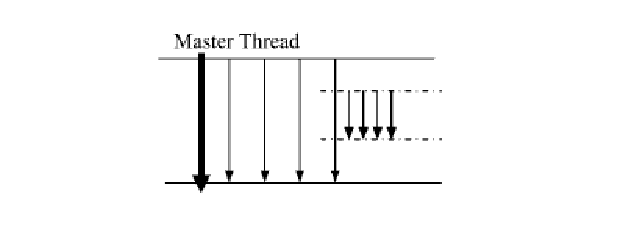
\includegraphics[width=0.9\textwidth]{openmp}
    \caption{openmp:Fork-Join模型}\label{fig:openmp}
    \vspace{\baselineskip}
    \end{figure}

    尽管有多种编程模式,但是并行编程模式通常可以归为四步:
    \begin{itemize}
    \item 任务划分,将整个问题和求解的功能分成一些小的计算任务,
    \item 通信分析,将任务划分之后,任务之间需要通信来进行数据交换,需要确定交换的数据类型,数据,时间等,用来协调任务的执行
    \item 任务组合,根据性能要求和算法复杂度,实现复杂度等来在前两步的基础上进行任务组合,进一步优化。
    \item 计算结点映射,据定将那个任务规划到相应的处理器上,以达到最小化全局执行时间和通讯成本,最大化计算能力的目的。
    \end{itemize}
\subsection{并行计算-硬件分类}
    并行计算机的的硬件实现环境即并行计算环境,是直接影响并行计算赖以生存的基础,根据据名的
Flynn分类法,根据指令流与数据流的特点进行区别.指令是指执行的指令流;数据流是指指令调用的
数据流,如I/O流,即输入输出数据.可以把计算机系统分类成一下分类
    \begin{enumerate}
    \item 单指令流多数据流SISD
    \item 单指令流单数据流SIMD
    \item 多指令流多数据流MISD
    \item 多指令流单数据流MIMD
    \end{enumerate}
\subsubsection{SISD}
    SISD计算机是传统的单进程计算机,指令顺序执行,单次执行一条指令,并且只对单个数据流进行处理
\subsubsection{SIMD}
    向量处理机是典型的SIMD并行机.向量机利用流水线的概念,将计算机的指令执行拆分开,分为多段,
每个流水线的不同时间段处理不同的数据流,通过时间上的重叠实现效率叠加.向量处理机在并行计算机的
发展历史上起到了推动的作用,由于后期性价比不高,加之处理器性能的不断增强,向量处理机推出了历史
舞台。SIMD结构示意图\cite{Hufeng}~\ref{fig:simd}。
    \begin{figure}[htbp]
    \centering
    \includegraphics[width=0.9\textwidth]{simd}
    \caption{SIMD结构示意图}\label{fig:simd}
    \vspace{\baselineskip}
    \end{figure}
\subsubsection{共享存储的MIMD并行机}
    共享存储MIMD并行多处理机,通过高速互联网络共享一个统一的内存空间,通过内存数据实现处理机
之间的协调.对于各个计算结点,每个计算节点可以执行不同的执行程序或者相同的执行程序,但是数据流
不同,以实现不同的数据处理和计算任务.各个结点的通信可以通过共享存储实现,这种结构方便并行程序的
编写,执行效率高.但是当结算节点较多时,当处理器太多时,会加重内存的竞争,这时可以通过告诉缓冲
高速缓冲技术等来实现数据的高速交换.
\subsubsection{分布存储的MIMD并行机}
    由于共享存储的MIMD并行机的特定性能瓶颈,分布存储MIMD的并行机开始有所应用.各个计算结点
有自己的局部存储器,结点之间通过消息传送进行联系,各个计算节点只能访问本身的局部存储器,无法
和无权限访问其他计算节点的存储器.各个计算节点之间消息传递进行联系.各个并行节点至今实际上是独立的,所以分布式存储并行机有良好的扩展性,可以通过增加并行处理机
的数量,来提高计算能力.各个计算结点通过相互通信,而消息传递对程序员不透明,所以编程难度增加。MIMD结构示意图~\ref{fig:mimd}

    并行计算机集群(Cluster)是分布存储的MIMD并行机重要表现形式,可以由一组相互独立的计算机在网络互联中分别以单一的系统方式
管理,提供稳定,可靠的服务。当Cluster内的某个结点发生故障时,可以由其他结点接替其的计算任务。Cluster具有自由伸缩,高度可
管理,高可用,高性价比等诸多优点,是在当前情况下大规模科学工程计算,如并行计算的非常理想的平台。Cluster的体系架构如图
~\ref{fig:cluster}
    \begin{figure}[htbp]
    \centering
    \includegraphics[width=0.8\textwidth]{mimd}
    \caption{MIMD结构示意图}\label{fig:mimd}
    \vspace{\baselineskip}
    \end{figure}

    \begin{figure}[htbp]
    \centering
    \includegraphics[width=0.8\textwidth]{cluster}
    \caption{集群体系结构示意图}\label{fig:cluster}
    \vspace{\baselineskip}
    \end{figure}

\subsection{并行计算-计算粒度划分}     
    \begin{enumerate}
    \item 子任务级的并行:不同程序功能的运行到不同的结点,不同程序功能差别较大时,不容易实现负载均衡
    \item 数据级的并行: 将要求解的问题的输入数据进行划分,每个计算节点负责不同的输入数据部分,由主进程
收集每个计算节点的计算数据
    \end{enumerate}



\section{并行计算程序性能评价}
    对于给定并行问题需求和特定解决方案,可以构造出不同的算法。如何衡量并行计算的性能成为需要考虑的问题,评价并行算法的优劣
,除了以下3个主要指标以外,还有算法时间复杂度和空间复杂度等。通常情况下,时间复杂度与算法优劣有关,空间复杂度与算法规模有关。
\subsection{并行程序执行时间}
    指的是从并行程序开始执行到结束执行所用的时间间隔,可以进一步分解为CPU计算时间,通信时间,进程同步开销时间,进程同步
导致的空闲等待时间。CPU计算时间为主要指标,主要时指程序指令本身执行所占用的时间。    
\subsection{加速比}
加速比做为衡量并行计算性能的重要指标之一,可以衡量并行计算的性能.加速比的公式,
    \[  S[N] = \frac{T_1}{T_N}  \]
其中N是指参与并行计算的CPU数量;$T_1$表示程序在单cpu上运行串行算法所需要的时间,也可以理解为并行算法在单个处理器执行的时间,
$T_N$表示程序在N个CPU上运行所需要的时间 ,S(N)为加速比。
    
    通常情况下,程序并不是所有部分都是可以被并行的,会存在着串行部分和可被并行的部分,设程序的串行部分为f,T1为并行算法在
单个处理器上执行的时间,则
\[ T_1 = fT_1+(1-f)T_1\]
\[ T_N = fT_1+(1-f)\frac{T_1}{N}\]

    所以加速比为
    $$S(N)=\frac{1}{f+\frac{1-f}{N}} = \frac{N}{Np+1-f} \leq \frac{1}{f} $$
    可见一个程序只要存在串行部分,即无论采用多少数量的处理结点,其加速系数都会不大于10,这就是$Amdahl$定理。 同时,由于进程
见间通讯造成的时间损失,所以通常加速比无法等于计算机结点的数目,只能接近于计算机节点的数目。S(N)越大,说明并行计算的性能越好
,处理效率越高, 但是S(N)与计算机的数目也有直接的关系,为了更好地衡量并行计算的性能,也可采用算法的并行效率指标。
\subsection{效率}
一般地,$T_N = \frac{T_1}{N}$,所以有$E_N <= 1 $ ,$E_N$越接近于1,说明并行效果越好,

    并行算法的成本主要为时间成本,等于并行机各处理器上运行时间的总和,计算公式可表达为
    
    \[ TimeCost=PxT_p  \]

